% Chapter X

\chapter{Caso di Studio sulle stazioni Dell'Abruzzo} % Chapter title
Il metodo proposto è valido per una grande varietà di assets. Tuttavia in questo lavoro è stato testato sulle stazioni e successivamente sulle linee ferroviarie del territorio abruzzese. 
L'Abruzzo è prevalentemente montuoso (65\%) e collinare (34\%) \cite{abruzzo}. La pianura (1\%) è costituita soltanto da una stretta fascia costiera lungo il litorale (Figura \ref{abruzzo_map}).

\begin{figure}[h]
	\centering
	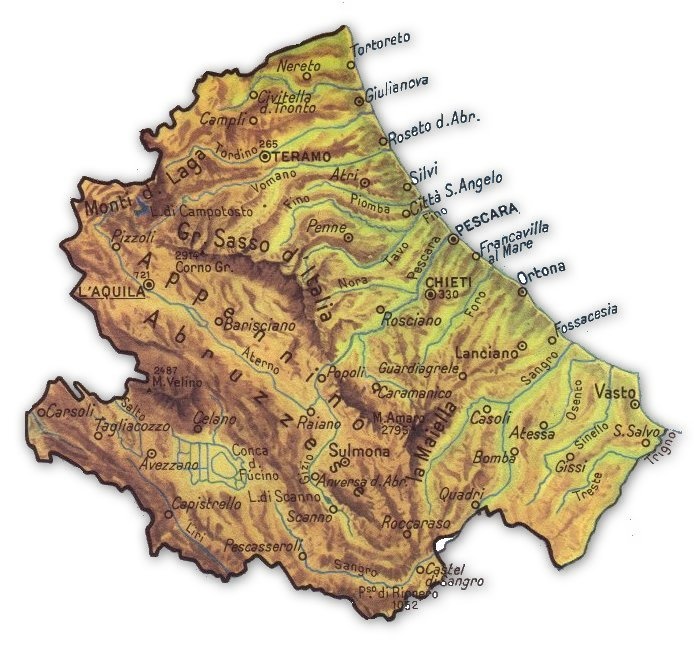
\includegraphics[width=0.6\textwidth]{images/abruzzo_disegno}
	\caption{Mappa dell'Abruzzo.}
	\label{abruzzo_map}
\end{figure}

Il territorio è particolarmente soggetto al rischio frana, com'è possibile osservare nella tabella \ref{tab:riassunto_frane}, dove i numeri delle frane verificatesi (accanto alla tipologia) sono davvero elevati. Inoltre tali frane sono quelle censite, quindi è molto probabile che il numero reale sia di gran lunga maggiore.

\begin{table}[h]
	\centering
	\begin{tabular}{|l|c|c|}
		\hline
		\multicolumn{1}{|c|}{\cellcolor{gray!50} \textbf{TIPO DI MOVIMENTO}} & {\cellcolor{gray!50}\textbf{NUM FRANE}} & {\cellcolor{gray!50} \textbf{\%}} \\ \hline
		Crollo/ribaltamento & 128  & 1,51   \\ \hline
		Scivolamento rotazionale/traslativo  & 3.401  & 40,05                              \\ \hline
		Espansione                                                                                      & 2                                        & 0,02                               \\ \hline
		Colamento lento                                                                                 & 2.364                                    & 27,84                              \\ \hline
		Colamento rapido                                                                                & 704                                      & 8,29                               \\ \hline
		Sprofondamento                                                                                  & 1                                        & 0,01                               \\ \hline
		Complesso                                                                                       & 1.331                                    & 15,67                              \\ \hline
		DGPV                                                                                            & 92                                       & 1,08                               \\ \hline
		Aree soggette a crolli/ribaltamenti diffusi                                                     & 63                                       & 0,74                               \\ \hline
		Aree soggette sprofondamenti diffusi                                                            & 6                                        & 0,07                               \\ \hline
		Aree soggette a frane superficiali diffuse                                                      & 257                                      & 3,03                               \\ \hline
		n.d. (tipo non determinato)                                                                     & 144                                      & 1,69                               \\ \hline
	\end{tabular}
	\caption{Le frane censite verificatesi in Abruzzo 	\cite{d200718}.}
	\label{tab:riassunto_frane}
\end{table}


Per questo motivo il territorio abruzzese è sicuramente un caso di studio interessante.
I dati su cui si è lavorato sono i seguenti:
\begin{enumerate}
	\item geo\_area: rappresenta la GEOAREA, ovvero la porzione di territorio di interesse;
	\item railway\_stations: concerne le stazioni appartenenti alla rete ferroviaria abruzzese;
	\item railway\_routes: riguarda le linee ferroviarie abruzzesi;
	\item abruzzo\_raster: i dati raster del territorio abruzzese.
\end{enumerate}
I files geo\_area, railway\_stations e railway\_routes sono degli shapefile. Il file raster abruzzo\_raster è stato utilizzato al fine di ricavarsi le curve di livello dell'intera geo\_area. Nell'appendice A è possibile leggere una descrizione dettaglia delle procedura della creazione del dataset, ovvero il modo in cui gli shapefile sono stati importati all'interno della base di dati e poi utilizzati.
Per tutta la fase di sperimentazione del metodo è stato utilizzato il software \textbf{PostgresSQL} con l’estensione spaziale \textbf{PostGIS}. In questo ambiente sono stati creati la base di dati, le viste le user defined function (UDF) e sono stati importati gli shapefile. Il software \textbf{QGIS} è stato utilizzato per visualizzare i dati dalle tabelle della basi dati. Il programma è in grado di visualizzare contemporaneamente, su più layers, i dati provenienti da diverse tabelle. In figura \ref{qgis} si possono vedere i dati importati visualizzati all'interno del software QGSIS. E' possibile riconoscere i confini dell'Abruzzo e le stazioni ferroviarie (pari a 114) rappresentate con dei pallini di colore rosso.

\begin{figure}[h]
	\centering
	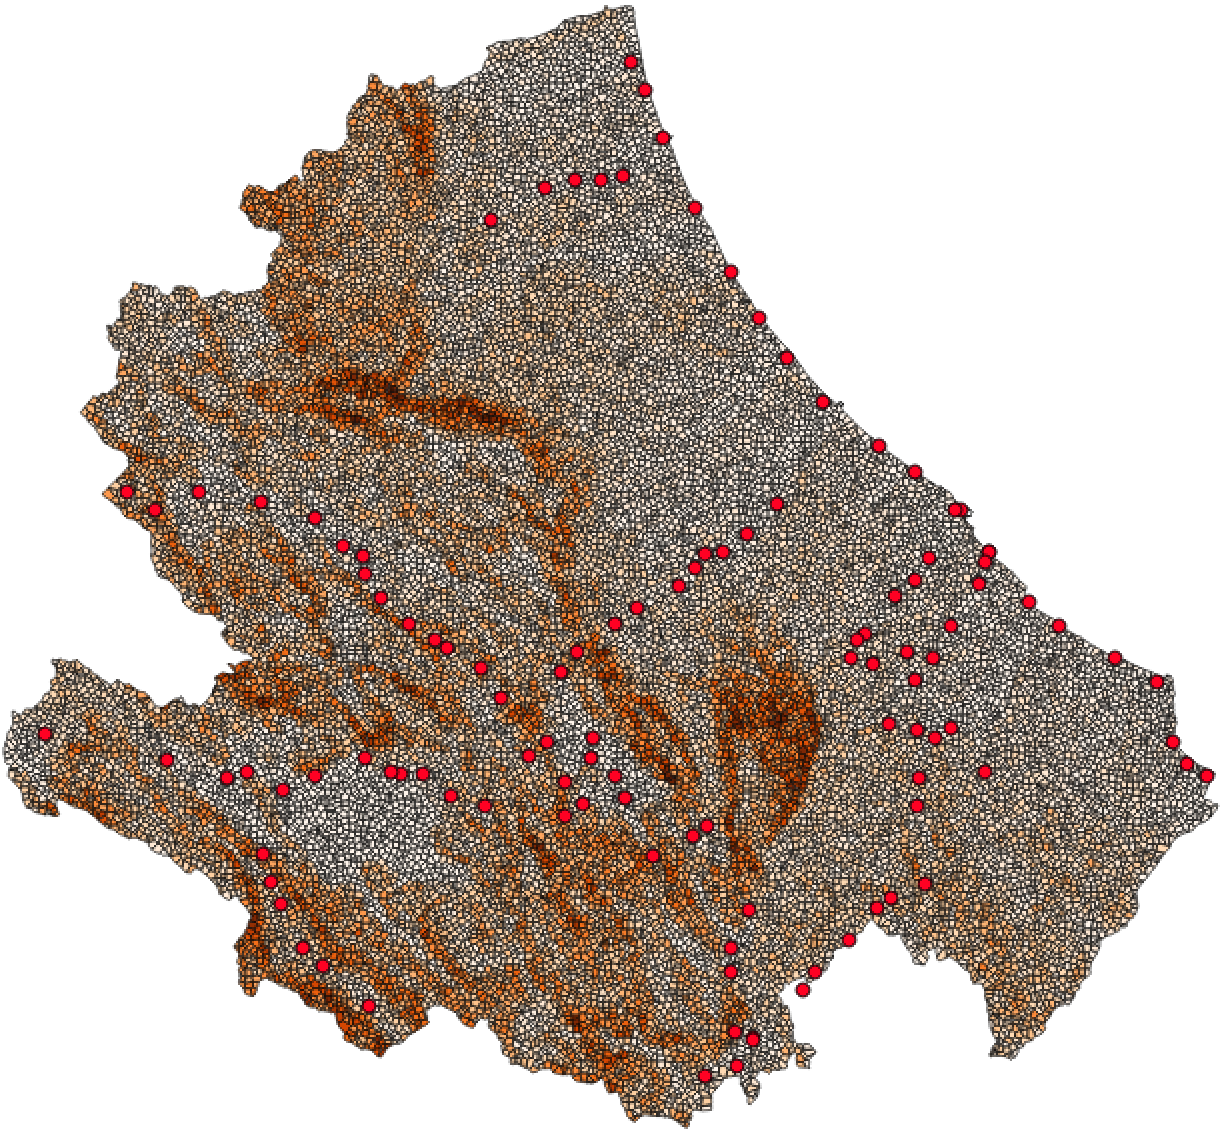
\includegraphics[width=0.6\textwidth]{images/dati_abruzzo_stazione}
	\caption{Rendering dei dati attraverso QGIS.}
	\label{qgis}
\end{figure}

I dati raster permettono inoltre una visualizzazione 3D del dataset all'interno del browser installato di default sulla macchina. Ciò è possibile attraverso il plugin \textbf{Qgis2threejs} di QGIS. Questa estensione è molto utile per la validazione e valutazione del metodo illustrate nella sezione 7.

\begin{figure}[h]
	\centering
	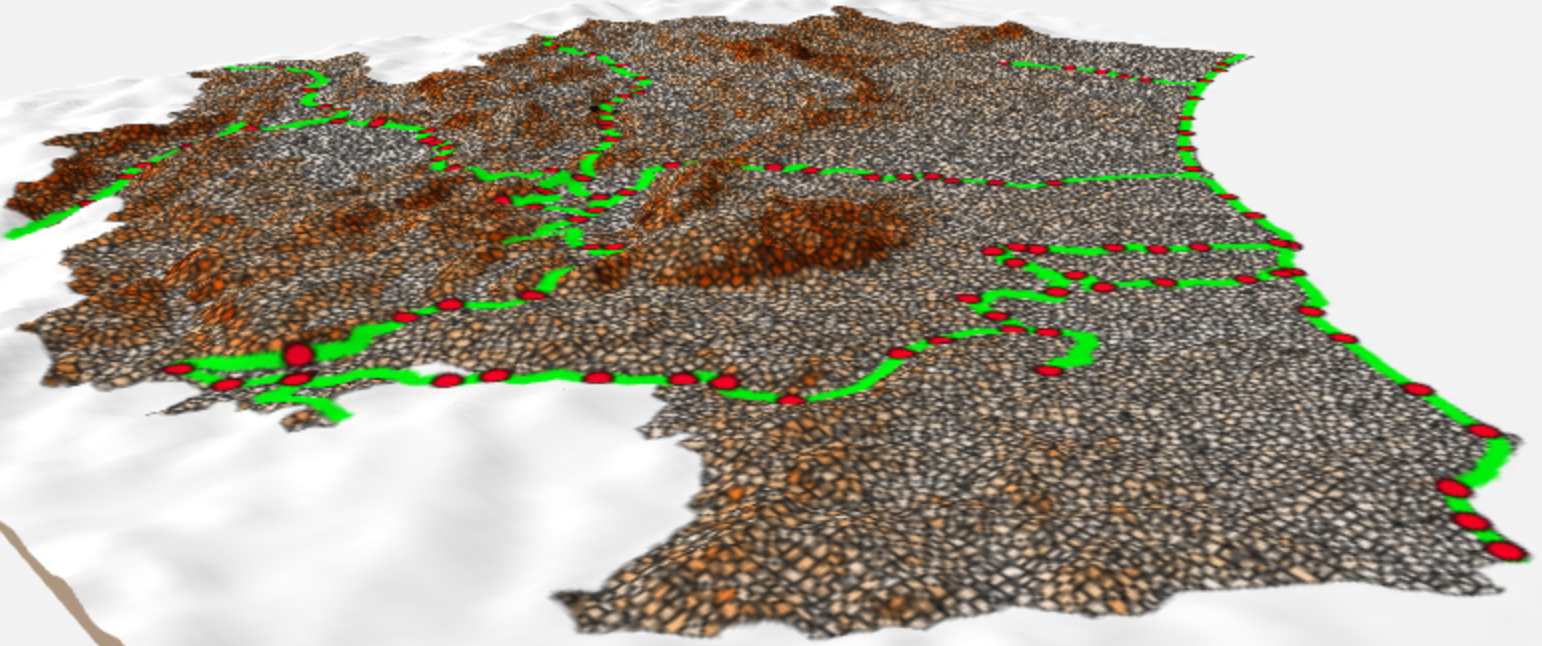
\includegraphics[width=0.7\textwidth]{images/Threejs}
	\caption{Rendering 3D dei dati iniziali attraverso il plugin Qgis2threejs di QGIS.}
	\label{threejs}
\end{figure}